\newcommand{\UTxOEpState}{\type{UTxOEpState}}
\newcommand{\Accnt}{\type{Accnt}}
\newcommand{\AccntEnv}{\type{AccntEnv}}
\newcommand{\AccntState}{\type{AccntState}}
\newcommand{\StPlCleanEnv}{\type{StPlCleanEnv}}
\newcommand{\StPlCleanState}{\type{StPlCleanState}}
\newcommand{\NewProtoConstsEnv}{\type{NewProtoConstsEnv}}
\newcommand{\NewProtoConstsState}{\type{NewProtoConstsState}}
\newcommand{\EpochEnv}{\type{EpochEnv}}
\newcommand{\EpochState}{\type{EpochState}}
\newcommand{\BlocksMade}{\type{BlocksMade}}
\newcommand{\Distr}{\type{Distr}}

\newcommand{\obligation}[4]{\fun{obligation}~ \var{#1}~ \var{#2}~ \var{#3}~ \var{#4}}
\newcommand{\reward}[5]{\fun{reward}~ \var{#1}~ \var{#2}~ \var{#3}~ \var{#4}~ \var{#5}}
\newcommand{\isActive}[4]{\fun{isActive}~ \var{#1}~ \var{#2}~ \var{#3}~ \var{#4}}
\newcommand{\activeStake}[5]{\fun{activeStake}~ \var{#1}~ \var{#2}~ \var{#3}~ \var{#4}~ \var{#5}}
\newcommand{\poolRefunds}[3]{\fun{poolRefunds}~ \var{#1}~ \var{#2}~ \var{#3}}

In this chapter we discuss the ledger state updates that take place at the epoch
boundary. These are necessary updates that are not triggered by a transaction.
It is impractical and unnecessary to perform the calculations and updates we
describe below every slot. The main state updates that take place at the boundary
are of an accounting nature, calculating new values for the various accounts
on the ledger (treasury, reserves, rewards, fees).

However, it is also when
pools scheduled for retirement at this boundary are removed from the ledger.
In addition, if there is an update planned for any of the protocol parameters,
it may only take place at the epoch boundary, and results in a ledger state
update, which we also give the details of in this chapter.
Note that witnessing here is not necessary because there is no data to sign
in the signal.

We introduce a two new derived types in this chapter. $\BlocksMade$ (see
Figure~\ref{fig:epoch-defs}), which represents the number of blocks made by
the blockchain this epoch associated to a particular stake key. The type
$\Distr$ is a finite map that pairs a hash key with a fraction. This fraction
is meant to represent the portion of the total stake corresponding to a key,
thus this type is used to give the stake distribution.

We also introduce two lookup functions. The map $\fun{stakeHK}$ looks up the
hash key at a base address, and the map $\fun{stakePtr}$ looks up the pointer
at a given pointer address.

The next three functions ($\fun{movingAvgWeight}$, $\fun{movingAvgExp}$, and
$\fun{globalPool}$) in the figure return a specific subset of parameters
in the set of protocol parameters (stake pool-specific parameters, respectively)
needed for performing rewards calculations.

%%
%% Figure - Epoch Abstract Types
%%
\begin{figure}[htb]
  \emph{Derived types}
  %
  \begin{equation*}
    \begin{array}{r@{~\in~}l@{\qquad=\qquad}lr}
      \var{prod}
      & \BlocksMade
      & \HashKey \mapsto \mathbb{N}
      & \text{blocks made in the epoch} \\
      \var{distr}
      & \Distr
      & \HashKey \mapsto [0,1]
      & \text{stake distribution} \\
    \end{array}
  \end{equation*}


  \emph{Abstract functions}
  %
  \begin{equation*}
    \begin{array}{r@{~\in~}lr}
      \fun{stakeHK} & \Addr_{base} \to \HashKey
      & \text{base address hashkey}\\
      \fun{stakePtr} & \Addr_{ptr} \to \Ptr
      & \text{pointer address pointer}\\
      \fun{movingAvgWeight} & \PParams \to [0, 1]
      & \text{moving average weight}\\
      \fun{movingAvgExp} & \PParams \to [0, 1]
      & \text{moving average exponent}\\
      \fun{globalPool} & \PParams \to \mathbb{R}_{>0}\times\mathbb{N}
      & \text{global pool parameters}\\
      \fun{globalAccntng} & \PParams \to [0,1] \times [0, 1]
      & \text{global accounting parameters}\\
      \fun{poolCosts} & \StakePool \to \Coin\times [0,1] \times \Coin
      & \text{pool cost parameters}\\
    \end{array}
  \end{equation*}
  \caption{Epoch definitions}
  \label{fig:epoch-defs}
\end{figure}

\subsection{Stake Distribution Calculation}
\label{sec:stake-dist}

One of the main characteristics of a proof-of-stake cryptocurrency is stake
distribution calculation. This calculation is performed at the epoch boundary.
We give the stake distribution calculations and related functions in
Figure~\ref{fig:functions:stake-distribution}.

The $\fun{baseStake}$ generates a finite map that pairs a staking key
associated to a base address with the coin value at that address as recorded
in the UTxO on the ledger. Note that this is a map indexed by any staking keys,
which every base address has (but not all of these are registered and delegating).
After registering a stake key, the base address is added alongside the
coin value associated to it in $outs$ (the outputs record currently in the
ledger UTxO).

The map
$\fun{ptrStake}$ generates a similar finite map for coin values at a given
pointer address in the UTxO outputs set, indexed the stake keys the given
pointer address is associated with.
This is a key and coin value pair finite map for only registered stake keys.

The $\fun{stake}$ map is a union of all the stake (both active and inactive) in
both of these finite
maps, $\fun{baseStake}$ and the $\fun{ptrStake}$.
The next step of calculating stake distribution is to filter the hash keys in
the $\fun{stake}$ finite map.
We want only those (stake) keys for which stake
from the $\fun{baseStake}$ and the $\fun{ptrStake}$ calculations is active, i.e.
for which the $\fun{isActive}$ filter is true.
For a hash key, its stake is active (i.e. $\fun{isActive}$) whenever it is a
registered stake key
and it is delegating to some registered stake pool.

The finite map output of the function $\fun{activeStake}$ gives the subset of
all the \textit{active} stake computed by $\fun{stake}$.
These stake-related calculations are used in the calculation of rewards.

%%
%% Figure - Functions for Stake Distribution
%%
\begin{figure}[htb]
  \begin{align*}
      & \fun{baseStake} \in \powerset{\TxOut} \to \powerset{(\HashKey \times \Coin)}
      & \text{base address stake} \\
      & \fun{baseStake}~{outs} = \\
      & ~~ \{(hk, c) \mid a\in\Addr_{base} \land (a, c) \in outs \land \fun{stakeHK}~a = hk \}
      \nextdef
      & \fun{ptrStake} \in \powerset{\TxOut} \to (\Ptr \mapsto \HashKey)
          \to \powerset{(\HashKey \times \Coin)}
      & \text{pointer address stake} \\
      & \fun{ptrStake}~{outs}~{ptrs} = \\
      & ~~ \{(hk, c) \mid a\in\Addr_{ptr} \land (a, c) \in outs \land (\fun{stakePtr}~a)\mapsto hk \in ptrs \}
      \nextdef
      & \fun{stake} \in \powerset{\TxOut} \to (\Ptr \mapsto \HashKey)
          \to \powerset{(\HashKey \times \Coin)}
      & \text{potential stake} \\
      & \fun{stake}~{outs}~{ptrs} = (\fun{baseStake}~{outs}) \cup (\fun{ptrStake}~{outs}~{ptrs})
      \nextdef
      & \fun{isActive} \in \HashKey \to \Allocs \to (\HashKey \mapsto \HashKey) \to \Allocs \to \mathbb{B}
      & \text{active stake} \\
      & \isActive{v_{sk}}{stkeys}{delegs}{stpools} = \exists \var{v_{p}}\\
      & ~~ \var{v_{sk}} \in \dom stkeys
              \land \var{v_{sk}}\mapsto\var{v_{p}} \in delegs
              \land \var{v_{p}} \in \dom \var{stpools}
      \nextdef
      & \fun{activeStake} \in \powerset{\TxOut} \to (\Ptr \mapsto \HashKey) \to \Allocs\\
      & ~~\to (\HashKey \mapsto \HashKey) \to \Allocs \to (\HashKey \mapsto \Coin)
      & \text{active stake holdings} \\
      & \activeStake{outs}{ptrs}{stkeys}{delegs}{stpools} = \\
      & ~~ \left\{
             hk\mapsto \sum_{hk\mapsto c}c
             ~\Big\vert~
             \begin{array}{r}
             (\isActive{hk}{stkeys}{delegs}{stpools}) \\
             \land (hk, c) \in (\fun{stake}~{outs}~{ptrs})
             \end{array}
           \right\}
  \end{align*}
  \caption{Functions used in Stake Distribution}
  \label{fig:functions:stake-distribution}
\end{figure}

\subsection{Accounting Functions}
\label{sec:acc-fun}

In Figure~\ref{fig:functions:epoch}, we give the functions used in the deposit
calculations at the boundary. Here we introduce the function $\fun{obligation}$
that gives the value of the total possible (decayed) refunds for both individual
and pool deposits in a given slot number.

Next, we give the type of the function used to calculate additional rewards that
will become available to be claimed after the boundary. This function is denoted
$\fun{reward}$, and depends on this epoch's blocks, protocol parameters, the
delegation and pool states, and existing rewards unclaimed in the previous
epoch.  The $\fun{reward}$ function updates the existing records of the
unclaimed coin values by adding newly accumulated rewards in this epoch to the
value in each reward address.

The function $\fun{poolRefunds}$ is used to calculate the total refunds
that must be distributed
for stake pools scheduled to retire at an epoch boundary. Note that this
calculation takes a slot number as a parameter because that is the type of value
needed for the decay calculation, but will only ever be invoked
when the slot number is the last before the boundary.

The map $\fun{poolRefunds}$ uses the pool decay parameters in $\PParams$
to assign a refund to each pool key in the set of pools scheduled for retirement
at the epoch boundary.

%%
%% Figure - Functions for Epoch Rules
%%
\begin{figure}[htb]
  \begin{align*}
      & \fun{obligation} \in \PParams \to \Allocs \to \Allocs \to \Slot \to \Coin
      & \text{total possible refunds} \\
      & \obligation{pp}{stkeys}{stpools}{cslot} =\\
      & \sum\limits_{(\_ \mapsto s) \in \var{stkeys}}
        \refund{d_{\mathsf{val}}}{d_{\min}}{\lambda_d}{(\slotminus{cslot}{s})} \\
      & + \sum\limits_{(\_ \mapsto s) \in \var{stpools}}
        \refund{p_{\mathsf{val}}}{p_{\min}}{\lambda_p}{(\slotminus{cslot}{s})} \\
      &
      \begin{array}{lr@{~=~}l}
        \where
          & (\dval,~d_{\min},~\lambda_d) & \fun{decayKey}~\var{pp}\\
          & (p_{\mathsf{val}},~p_{\min},~\lambda_p) & \fun{decayPool}~\var{pp}\\
      \end{array}\\
      \nextdef
      & \fun{poolRefunds} \in \PParams \to \Allocs \to \Slot \to (\HashKey \mapsto \Coin)
      & \text{pool refunds} \\
      & \poolRefunds{pp}{retiring}{cslot} = \\
      & \bigcup_{\var{hk}\mapsto s\in\var{retiring}}
          \var{hk}\mapsto( \refund{p_{\mathsf{val}}}{p_{\min}}{\lambda}{(\slotminus{cslot}{s})} ) \\
      &
        \where (p_{\mathsf{val}},~p_{\min},~\lambda_p) = \fun{decayPool}~\var{pp}\\
  \end{align*}
  \caption{Functions used in Accounting}
  \label{fig:functions:epoch}
\end{figure}

\subsection{Rewards Distribution}
\label{sec:reward-dist}

We now discuss reward distribution calculation that happens at the epoch boundary.
Functions used in reward calculations are presented in
Figure~\ref{fig:functions:rewards}. The reward calculation below is done as part of the
epoch boundary accounting to update the various accounting fields on the ledger,
see Section~\ref{sec:acc-trans}. In the subsequent calculations, we use the
following variables, sourced as indicated (listed here for reference):

\begin{itemize}
\item[] From the delegation state:
\item $\var{avgs}$ stores the (moving) average for each
stake pool
\item $\var{poolParam}$ stores stake pool-specific parameters
\item $\var{delegs}$ stores delegations as stake and pool key pairs \medskip

From the boundary accounting transition context:
\item $\var{prod}$ gives the number of blocks made by each stake pool
this epoch, with $n$ representing the number of blocks corresponding to the
given pool \medskip

Calculated as part of epoch boundary accounting, see
Section~\ref{sec:acc-trans}:
\item $\var{R} \in \Coin$ is the total available rewards for the epoch (in ADA) \medskip

From protocol (pool-related) constants:
\item $n_{opt} \in \mathbb{N}$ is the optimal number of saturated stake pools (which the system
tends to by protocol design)
\item $\var{a_0} \in [0, \infty)$ is a parameter determining leader-stake
influence on pool rewards
\item $\gamma$ is the moving average exponent constant \medskip

From pool-specific parameters denoted $\var{pool}$, associated to a specific
hash key in $\var{poolParam}$:
\item $c \in \Coin$ is the pool costs
\item $m \in [0,1]$ is the stake pool margin
\item $p \in \Coin$ is the pledge a stake key registering a pool defines (via
the registration certificate)\medskip

Calculated by the functions defined in this section using the variables above:
\item $\var{z_0} := 1/n_{opt}$ is the size of a saturated pool
\item $\var{active}$ is the finite map associating a stake key to all the
active stake belonging to it
\item $s \in [0,1]$, or $t$, is the relative stake associated to a specific stake key
(i.e. the value associated to it in $\var{active}$ stake, normalized)
\item $\var{tot} \in \Coin$ is the sum total of all the $\var{active}$ stake
\item $\var{actgr}$ is the subset of the total $\var{active}$ stake
for which its stake key delegates to a given pool
\item $\var{pactive}$ is the finite map of all the subsets of $\var{actgr}$,
each associated to its pool key
\item $\sigma \in [0,1]$ is the total relative stake of a pool (expressed as a fraction of
the total stake, which is a sum of the relative member's stake)
\item $p_r \in [0,1]$ is the relative pledge of a given pool, calculated by normalizing $p$
\item $\overline{N} \in \mathbb{R}$, for a given pool, is the expectated value of the number
of slots that the pool will be elected as leader on average
\item $\var{maxP} \in \Coin$ is the maximum stake that could be received by a particular
pool
\item $\var{\hat{f}}$ is the pool rewards
\item $\var{avg}$ is the relative moving average for a given pool calculated for
the current epoch
\end{itemize}

The function $\fun{maxPool}$ gives the maximum possible amount of rewards a pool
can receive in an epoch. For a given pool, it is a coin value which is some fraction of
the total available rewards. This result depends additionally on the protocol
parameters, the pool's relative stake, and the pool's relative pledge.

The function $\fun{movingAvg}$ calculates the new moving average for a
given stake pool based on protocol parameters, pool's block production, and
the moving average of this pool in the previous epoch.

Next, the function $\fun{poolRew}$ gives the total rewards available to be distributed
to the members of the given pool. This value is based on protocol parameters,
the pool's block production, moving average, election expectation, and the maximum
possible rewards for this pool.

%%
%% Figure - Functions for the Reward Calculation
%%
\begin{figure}[htb]
  \begin{align*}
      & \fun{maxPool} \in \PParams \to \Coin \to [0, 1] \to [0,1] \to \Coin
      & \text{max pool reward} \\
      & \fun{maxPool}~\var{pp}~\var{R}~\sigma~\var{p_r} = \\
      & ~~~\floor*{
           \frac{R}{1 + a_0}
           \cdot
           \left(\sigma' + p'\cdot a_0\cdot\frac{\sigma' - p'\frac{z_0-\sigma'}{z_0}}{z_0}\right)} \\
      & ~~~\where \\
      & ~~~~~~~(a_0, n_{opt}) = \fun{globalPool}~pp \\
      & ~~~~~~~z_0 = 1/n_{opt} \\
      & ~~~~~~~\sigma'=\min(\sigma,~z_0) \\
      & ~~~~~~~p'=\min(p_r,~z_0) \\
      \nextdef
      & \fun{movingAvg} \in \PParams \to \HashKey \to \mathbb{N} \to \mathbb{R} \\
      & ~~~\to \Distr \to [0, 1]
      & \text{moving average} \\
      & \fun{movingAvg}~\var{pp}~\var{hk}~\var{n}~\var{\overline{N}}~\var{avgs} = \\
      & \begin{cases}
        \frac{n}{\max(\overline{N}, 1)}
        & hk\notin \dom\var{avgs}\\
        \\
          \alpha\cdot\frac{n}{\max(\overline{N}, 1)}+(1-\alpha)\cdot\var{prev}
        & hk\mapsto\var{prev}\in\var{avgs}\\
        \end{cases} \\
      & ~~~\where \\
      & ~~~~~~~\alpha = \fun{movingAvgWeight}~pp \\
      \nextdef
      & \fun{poolRew} \in \PParams \to \HashKey \to \mathbb{N} \to \mathbb{R} \\
      & ~~~\to \Distr \to \Coin \to (\Coin \times [0, 1])
      & \text{pool reward} \\
      & \fun{poolRew}~\var{pp}~\var{hk}~\var{n}~\var{\overline{N}}~\var{avgs}~\var{maxP} =
      (\floor*{avg^\gamma\cdot \var{maxP}},~\var{avg})\\
      & ~~~\where \\
      & ~~~~~~~\gamma = \fun{movingAvgExp}~pp \\
      & ~~~~~~~\var{avg} = \fun{movingAvg}~\var{pp}~\var{hk}~\var{n}~\var{\overline{N}}~\var{avgs} \\
  \end{align*}
  \caption{Functions used in the Reward Calculation}
  \label{fig:functions:rewards}
\end{figure}

In Figure~\ref{fig:functions:reward-splitting}, we give the strategy for the
splitting of the rewards within a given pool. Note that the calculation of
the total value to be split within the pool is presented above, denoted $\fun{poolRew}$.

The portion of rewards allocated to the pool leader and those allocated to
the rest of the pool members is different. This portion is calculated based
on pool-specific parameters stored on the ledger, as well as
the pool's total stake and the individual stake of the key for which the rewards
are being calculated. The calculation for the pool
leader reward amount is given by the $\fun{leaderRew}$ function, and the
calculation for the reward amount for each other member is given by $\fun{memberRew}$.
Finally, $\fun{indivRew}$ puts these two calculations together to give the
reward amount for any pool member, using a boolean $\var{isLeader}$
as an input variable which indicates
whether a given member is the pool leader or not.

Here we also present the $\fun{groupByPool}$ map, which, given the active stake
belonging to each registered stake key,
as well as the current delegations, produces a
finite map indexed by the hash keys of pool leaders. Each $\var{leader}$ key is associated
with a subset of the active stake finite map. This associated subset
contains only the entries where the hash keys delegate to that pool
which the given leader is the leader of.

%%
%% Figure - Functions for the Reward Splitting
%%
\begin{figure}[htb]
  \begin{align*}
      & \fun{leaderRew} \in \Coin \to \StakePool \to [0, 1] \to [0, 1] \to \Coin
      & \text{pool leader reward} \\
      & \fun{leaderRew}~\hat{f}~\var{pool}~\sigma~\var{s} = \\
      & \begin{cases}
          \hat{f} & \hat{f} \leq c\\
          c + \floor*{(\hat{f} - c)\cdot\left(m + (1-m)\cdot\frac{s}{\sigma}\right) }&
          \text{otherwise.}
        \end{cases} \\
      & ~~~\where \\
      & ~~~~~~~(c, m, \_) = \fun{poolCosts}~pool \\
      \nextdef
      & \fun{memberRew} \in \Coin \to \StakePool \to [0, 1] \to [0, 1] \to \Coin
      & \text{pool member reward} \\
      & \fun{memberRew}~\hat{f}~\var{pool}~\sigma~\var{s} = \\
      & \begin{cases}
          0 & \hat{f} \leq c\\
          \floor*{(\hat{f} - c)\cdot(1-m)\cdot\frac{s}{\sigma}} &
          \text{otherwise.}
        \end{cases} \\
      & ~~~\where \\
      & ~~~~~~~(c, m, \_) = \fun{poolCosts}~pool \\
      \nextdef
      & \fun{indivRew} \in \Coin \to \StakePool \to [0, 1] \to [0, 1] \to \mathbb{B} \to \Coin
      & \text{pool individual reward} \\
      & \fun{indivRew}~\hat{f}~\var{pool}~\sigma~\var{s}~\var{isLeader} = \\
      & \begin{cases}
          \fun{leaderRew}~\hat{f}~\var{pool}~\sigma~\var{s} & \var{isLeader} \\
        \fun{memberRew}~\hat{f}~\var{pool}~\sigma~\var{s} & \text{otherwise.}
        \end{cases} \\
      \nextdef
      & \fun{groupByPool} \in (\HashKey \mapsto \Coin) \to (\HashKey \mapsto \HashKey) \\
      & ~~~\to
        \left(
        \HashKey \mapsto
        \left(
        \HashKey \mapsto \Coin
        \right)
        \right)
      & \text{pool individual reward} \\
      & \fun{groupByPool}~\var{active}~\var{delegs} = \\
      & ~~~\Big\{ leader \mapsto
      \{hk \mapsto c \mid hk \mapsto c \in active\} \\
      & ~~~~~~            \mid hk \mapsto leader\in\var{delegs} \Big\}
  \end{align*}
  \caption{Functions used in the Reward Splitting}
  \label{fig:functions:reward-splitting}
\end{figure}


Finally, the reward calculation is presented in
Figure~\ref{fig:functions:reward-calc}. The calculation is done pool-by-pool.
The map $\fun{rewardOnePool}$ calculates the rewards given out to each member
of a given pool (with leader identified by
the stake key $\var{poolHK}$). The active stake associated to each
pool member is passed to $\fun{rewardOnePool}$
via the $\var{actgr}$ variable, which is a subset of hash keys in this pool
paired with the stake associated with the keys.

This $\fun{rewardOnePool}$ map outputs a finite map and an $\var{avg}$
value. The finite map is indexed
by reward addresses. In particular, the subset of reward addresses corresponding
to registered keys delegating to the pool with leader $\var{poolHK}$.
A reward address of key $hk$ is paired with the individual reward value
produced by the $\fun{indivRew}$ map applied to relevant data passed to
$\fun{rewardOnePool}$ as well as the results of the $\fun{maxPool}$
and $\fun{poolRew}$ calculations. The $\var{avg}$ value for the stake pool
(i.e. the pool's ranking) is also calculated by the $\fun{poolRew}$ function.

The $\fun{reward}$ calculation itself uses the $\fun{rewardOnePool}$ function to
reward each pool's members and calculate the pool's moving averages. In order to
do this, it is given the following parameters:

\begin{itemize}
\item The number of blocks made by each key this epoch
\item The protocol parameters
\item The total coin value of rewards to be distributed this epoch
\item The full delegation state
\item The set of outputs in the UTxO on the ledger
\end{itemize}

The output of the $\fun{reward}$ calculation is a pair. The first component is
a finite map indicating the new rewards assigned to each reward address.
The second component is the record of every pool's updated moving average.

Within the $\fun{reward}$ calculation, the active stake corresponding to each
(active and delegating to an active pool) stake key, $\var{active}$, is
calculated by adding up the total active stake for that key currently on the
ledger. The entries of this finite map are then grouped into subsets by the pool
each stake key belongs to using the $\fun{groupByPool}$ mapping (to give the
$\var{pactive}$ value).

Next, a dataset of $\var{results}$ is generated by pairing each pool key with
the set of rewards calculated for each of the delegators to the pool with this
key, as well as the moving average for the pool. Both of these are calculated
using the $\fun{rewardOnePool}$ function.  To generate the final output of the
$\fun{reward}$ calculation, we take the union of the all the subsets of the
rewards records of individual keys from the range values of the $\var{results}$
map, and pair it with the union of all the pool keys (the domain of the
$\var{results}$) and the associated moving averages for these (the second
component of the range of the $\var{results}$ finite map).

\begin{note}
In the~\cite{delegation_design} document, Section 6.5.1, the values of individual
relative stake $s$ and pool relative stake $\sigma$ are calculated by
dividing the corresponding total values by total ADA (31, 000, 000, 000). In this
document, we normalize pool and individual stake, i.e. obtain $s$ and $\sigma$
by dividing by the sum total of \textit{all active stake} $tot$. We also calculate
the relative pledge in the same way, $p_r = p \div tot$.
\end{note}

%%
%% Figure - The Reward Calculation
%%
\begin{figure}[htb]
  \begin{align*}
      & \fun{rewardOnePool} \in \PParams \to \Coin \to \mathbb{N} \to \HashKey \to \StakePool\\
      & ~~~\to (\HashKey \mapsto \Coin)\to \Distr \to \Coin \to (\AddrRWD \mapsto \Coin)\times[0, 1]
      & \text{reward one pool} \\
      & \fun{rewardOnePool}~\var{pp}~\var{R}~\var{n}~\var{poolHK}~\var{pool}
        ~\var{actgr}~\var{avgs}~\var{tot} = \\
      & ~~~(\{ (\AddrRWD~hk)\mapsto ( \fun{indivRew}~\var{poolR}~\var{pool}
                                 ~(\sigma\div\var{tot})~(\var{c}\div\var{tot})~(hk ==\var{poolHK})) \\
      & ~~~~~~~\mid hk\mapsto c\in\var{actgr}\},~\var{avg})\\
      & ~~~\where \\
      & ~~~~~~~\var{pstake} = \sum_{\_\mapsto t\in\var{actgr}} t \\
      & ~~~~~~~\sigma = \var{pstake} \div tot \\
      & ~~~~~~~\var{\overline{N}} = \sigma * \slotsPer\\
      & ~~~~~~~(\_, \_, p) = \fun{poolCosts}~pool \\
      & ~~~~~~~p_{r} = p \div tot \\
      & ~~~~~~~maxP =
      \begin{cases}
          \fun{maxPool}~\var{pp}~\var{R}~\sigma~\var{p_r}&
              p \leq \var{pstake}\\
          0 & \text{otherwise.}
        \end{cases} \\
      & ~~~~~~~(\var{poolR},~\var{avg}) = \fun{poolRew}~\var{pp}~\var{hk}~\var{n}~\var{\overline{N}}~\var{avgs}~\var{maxP} \\
      \nextdef
      & \fun{reward} \in \BlocksMade \to \PParams \to \Coin \\
      & ~~ \to \DPState \to \UTxO \to (\AddrRWD \mapsto \Coin)\times\Distr
      & \text{staking rewards} \\
      & \fun{reward}~\var{prod}~\var{pp}~\var{R}~\var{dpstate}~\var{utxo} = \\
      & ~~~\left(
           \bigcup_{hk\mapsto(rew,~\_)\in\var{results}} hk\mapsto\var{rew},
           ~~\bigcup_{hk\mapsto(\_,~\var{avg})\in\var{results}} hk\mapsto\var{avg}
           \right)\\
      & ~~~\where \\
      & ~~~~~~~\var{outs} = \{out\mid\_\mapsto\var{out}\in\var{utxo}\} \\
      & ~~~~~~~\var{dstate},\var{pstate} = \var{dpstate} \\
      & ~~~~~~~\var{stkeys},\_,\var{delegs},\var{ptrs} = \var{dstate} \\
      & ~~~~~~~\var{stpools},\var{poolParam},\var{retiring},\var{avgs} = \var{pstate} \\
      & ~~~~~~~active = \activeStake{outs}{ptrs}{stkeys}{delegs}{stpools} \\
      & ~~~~~~~tot = \sum_{\_\mapsto c\in \var{active}}c \\
%      & ~~~~~~~stDistr = \left\{ hk\mapsto c \div tot \mid hk \mapsto c \in \var{active} \right\}\\
      & ~~~~~~~pactive = \fun{groupByPool}~\var{active}~\var{delegs} \\
      & ~~~~~~~pdata = \left\{
                         hk\mapsto (pool, n, actgr)  \mathrel{\Bigg|}
                          \begin{array}{r@{\mapsto}c@{~\in~}l}
                          hk & \var{pool} & \var{poolParam} \\
                          hk & \var{n} & \var{prod} \\
                          hk & \var{actgr} & \var{pactive} \\
                          \end{array}
                       \right\} \\
      & ~~~~~~~results = \{hk \mapsto \fun{rewardOnePool}~\var{pp}~\var{R}~\var{n}~\var{hk}
      ~\var{pool}~\var{actgr}~\var{avgs}~\var{tot}
                         \mid \\
      &\qquad \qquad \qquad \qquad hk\mapsto(pool, n, actgr)\in\var{pdata} \}
  \end{align*}
  \caption{The Reward Calculation}
  \label{fig:functions:reward-calc}
\end{figure}

\clearpage

\subsection{Accounting Epoch Transition}
\label{sec:acc-trans}

The Figure~\ref{fig:ts-types:accnt} gives the definitions related to epoch
boundary ledger accounting. The figure lists the accounting fields, denoted by
$\Accnt$, which include $\var{treasury}$ (the amount of coin currently in
circulation, but not on the UTxO and not designated for rewards),
$\var{reserves}$ (the amount of coin
not yet in circulation),
and $\var{rewardPot}$ (the total amount available for distribution of rewards).
The figure also gives the set of necessary accounting environment
variables, $\AccntEnv$, and the accounting state, $\AccntState$, which includes
the delegation state and the accounting fields. The accounting state transition
type, as all transition types in this chapter, has no signal.

%%
%% Figure - Accounting Defs
%%
\begin{figure}[htb]
  \emph{Accounting Fields}
  \begin{equation*}
    \Accnt =
    \left(
      \begin{array}{r@{~\in~}ll}
        \var{treasury} & \Coin & \text{treasury pot}\\
        \var{reserves} & \Coin & \text{reserve pot}\\
        \var{rewardPot} & \Coin & \text{reward pot}\\
      \end{array}
    \right)
  \end{equation*}
  %
  \emph{Accounting environment}
  \begin{equation*}
    \AccntEnv =
    \left(
      \begin{array}{r@{~\in~}ll}
        \var{slot} & \Slot & \text{last slot of epoch}\\
        \var{pp} & \PParams & \text{protocol parameters}\\
        \var{blocksMade} & \BlocksMade & \text{blocks made in the epoch}\\
      \end{array}
    \right)
  \end{equation*}
  %
  \emph{Accounting States}
  \begin{equation*}
    \AccntState =
    \left(
      \begin{array}{r@{~\in~}ll}
        \var{accnt} & \Accnt & \text{accounting}\\
        \var{dstate} & \DState & \text{delegation state}\\
        \var{pstate} & \PState & \text{pool state}\\
        \var{utxoSt} & \UTxOState & \text{utxo state}\\
      \end{array}
    \right)
  \end{equation*}
  %
  \emph{Accounting transitions}
  \begin{equation*}
    \_ \vdash
    \var{\_} \trans{accnt}{} \var{\_}
    \subseteq \powerset (\AccntEnv \times \AccntState \times \AccntState)
  \end{equation*}
  %
  \caption{Accounting transition-system types}
  \label{fig:ts-types:accnt}
\end{figure}


The accounting epoch boundary rule in Figure~\ref{fig:rules:accnt} is the rule
where the most attention to detail is required in order to adhere to the
preservation of value condition. In this rule, the funds in each of the
accounting variables, as well as the individual reward addresses, are adjusted
as follows:

\begin{itemize}
\item To the $\var{treasury}$ we add a fraction $\tau$ of the sum of
the fees accumulated from transactions this epoch, the decay amount
of all current deposits, the total reward pool, and the expansion (how much
coin is added to circulation each epoch)
\item A fraction $\rho$ of the $\var{reserves}$ comes into circulation (i.e.
is removed from $\var{reserves}$)
\item The value added to $\var{treasury}$ is removed from the $\var{rewardPot}$
\item The sum total of rewards accumulated for all addresses this epoch
is removed from the $\var{rewardPot}$
\item The accumulated fees, deposit decay, and circulation expansion is
added to the $\var{rewardPot}$
\item The rewards accumulated this epoch are distributed by
adding the amount computed for each reward address (by the $\fun{reward}$ calculation)
to the value of coin corresponding to that address
\item The $\var{avgs}$ value in the delegation state is re-calculated and
updated by the $\fun{reward}$ map also
\item The deposit pot is set to the current obligation.
\item The fee pot is set to zero.
\end{itemize}

Note that fees and deposit decay, above, are not explicitly removed from any account:
the fees come from transactions paying them, and are accounted for whenever
transactions are processed, and the deposit decay value comes from returning
smaller refunds for deposits than were paid upon depositing.

Recall also that in Section~\ref{sec:reward-dist}, we used $R$ to represent
the total available rewards. Here, we present the calculation of the value
passed to $\fun{rewards}$ as $R$, denoted $\var{availablePool}$ above.
This value is a fraction $1-\tau$ of the sum of fees collected this epoch, the
deposit decay, leftover rewards from
the previous epoch, and this epoch's circulation expansion. The rest of this
value (i.e. $\tau$) goes into the $\var{treasury}$, as stated above.

Figure \ref{fig:fund-preservation} captures the potential movement of funds
between these various locations during the epoch transition and transaction
processing. In particular, the red subgraph represents the inputs and outputs to
the ``total pot'' used during the epoch transition in Figure \ref{fig:rules:accnt}.

\begin{figure}[htb]
  \begin{center}
    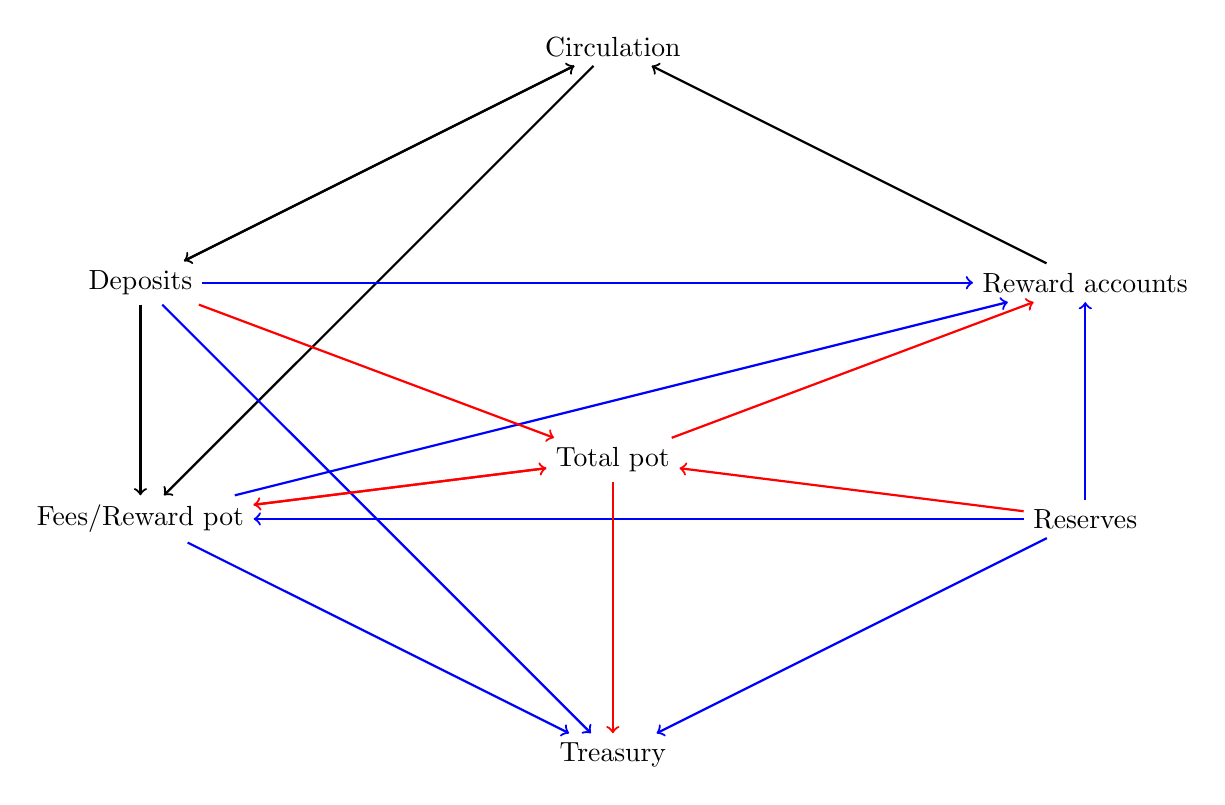
\begin{tikzpicture}
      [ x=30mm, y=30mm
      , direct/.style={black, draw}
      , implied/.style={blue, draw}
      , toTotPot/.style={red, draw}
      ]
    \node (C) at (3,3) {Circulation};
    \node (R) at (5, 1) {Reserves};
    \node (D) at (1, 2) {Deposits};
    \node (FR) at (1,1) {Fees/Reward pot};
    \node (RA) at (5, 2) {Reward accounts};
    \node (T) at (3,0) {Treasury};

    \draw[->, direct, thick]
    (C) edge (D)
    (C) edge (FR)

    (D) edge (C)
    (D) edge (FR)

    (RA) edge (C);

    \draw[->, implied, thick]
    (D) edge (RA)
    (D) edge (T)

    (FR) edge (T)
    (FR) edge (RA)

    (R) edge (FR)
    (R) edge (T)
    (R) edge (RA);

    \node (TP) at (3, 1.25) {Total pot};

    \draw[->, toTotPot, thick]
    (D) edge (TP)
    (FR) edge (TP)
    (R) edge (TP)

    (TP) edge (RA)
    (TP) edge (FR)
    (TP) edge (T);

  \end{tikzpicture}
  \end{center}
  \caption{Conservation of money}
  \label{fig:fund-preservation}
\end{figure}

%%
%% Figure - Accounting Rules
%%
\begin{figure}[htb]
  \begin{equation}\label{eq:accnt}
    \inference[Accounting]
    {
      {
      \begin{array}{r@{=}l}
        \rho, \tau & \fun{globalAccntng}~{pp} \\
        \var{obl} & \obligation{pp}{stkeys}{stpools}{slot} \\
        \var{decayed} & \var{deposits} - \var{obl} \\
        \var{expansion} & \floor*{\rho \cdot \var{reserves}} \\
        \var{totalPool} & \var{fees} + \var{decayed} + \var{rewardPot} + \var{expansion} \\
        \var{newTreasury} & \floor*{\tau \cdot \var{totalPool}} \\
        \var{availablePool} & \var{totalPool} - \var{newTreasury} \\
        \var{rewards'},~\var{avgs'} & \reward{blocksMade}{pp}{availablePool}{dpstate}{utxo}\\
        \var{paidRewards} & \sum\limits_{\_\mapsto c\in\var{rewards'}}c
      \end{array}
      }
    }
    {
      \begin{array}{l}
        \var{slot}\\
        \var{pp}\\
        \var{blocksMade}\\
      \end{array}
      \vdash
      \left(
        \begin{array}{r}
          \var{treasury} \\
          \var{reserves} \\
          \var{rewardPot} \\
          \var{stkeys} \\
          \var{rewards} \\
          \var{delegations} \\
          \var{ptrs} \\
          \var{stpools} \\
          \var{poolParam} \\
          \var{retiring} \\
          \var{avgs} \\
          \var{utxo} \\
          \var{deposits} \\
          \var{fees} \\
        \end{array}
      \right)
      \trans{accnt}{}
      \left(
        \begin{array}{rcl}
          \varUpdate{\var{treasury}} & \varUpdate{+} & \varUpdate{\var{newTreasury}} \\
          \varUpdate{\var{reserves}} & \varUpdate{-} & \varUpdate{\var{expansion}} \\
          \varUpdate{\var{availablePool}} & \varUpdate{-} & \varUpdate{\var{paidRewards}} \\
          \var{stkeys} \\
          \varUpdate{\var{rewards}} & \varUpdate{\unionoverridePlus} & \varUpdate{\var{rewards'}} \\
          \var{delegations} \\
          \var{ptrs} \\
          \var{stpools} \\
          \var{poolParam} \\
          \var{retiring} \\
          \varUpdate{\var{avgs'}} \\
          \var{utxo} \\
          \varUpdate{obl} \\
          \varUpdate{0} \\
        \end{array}
      \right)
    }
  \end{equation}
  \caption{Accounting Epoch inference rules}
  \label{fig:rules:accnt}
\end{figure}

\subsection{Epoch Boundary Pool Cleanup}
\label{sec:pool-clean}

Next, we discuss the epoch boundary pool retirement in
Figure~\ref{fig:ts-types:pool-clean}. The type of this transition is similar
to the other $\PState$ transition type we defined earlier, which is triggered
by a signal certificate,
however, this one has an empty signal (as it happens at the boundary).

%%
%% Figure - Pool Clean Defs
%%
\begin{figure}[htb]
  \begin{equation*}
    \_ \vdash \_ \trans{poolclean}{} \_ \in
    \powerset (\Slot \times \PState \times \PState)
  \end{equation*}
  %
  \caption{Pool Clean Transition}
  \label{fig:ts-types:pool-clean}
\end{figure}


We now present the pool-cleanup transition rule in Figure~\ref{fig:rules:pool-clean}.
This rule will be applied whenever there is one or more stake pools scheduled
to retire this epoch. If so, all of the entries in $\var{stpools}$,
$\var{poolParam}$, and $\var{retiring}$ which correspond to any of the hash keys
of the stake pools scheduled to retire this epoch are removed from
these variables.

It is important to note here that we \textit{do not} clean up delegations to
retired stake pools. While we do not allow registration to non-existent
stake pools (because that is a meaningless operation likely to be the result
of an error), delegating to a pool that was once active means that there may
be stake associated with this delegation. While this stake becomes inactive when
the pool is retired, the delegations to that pool must remain on the ledger
for potential future use.

%%
%% Figure - Pool Clean Rule
%%
\begin{figure}[htb]
  \begin{equation}\label{eq:pool-clean}
    \inference[Pool-Clean]
    {
      \var{retired} = \var{retiring}^{-1}~\var{(\epoch{slot})}
    }
    {
      \begin{array}{l}
        \var{slot}\\
      \end{array}
      \vdash
      \left(
        \begin{array}{r}
          \var{stpools} \\
          \var{poolParam} \\
          \var{retiring} \\
          \var{avgs} \\
        \end{array}
      \right)
      \trans{poolclean}{}
      \left(
        \begin{array}{rcl}
          \varUpdate{\var{retired}} & \varUpdate{\subtractdom} & \varUpdate{\var{stpools}} \\
          \varUpdate{\var{retired}} & \varUpdate{\subtractdom} & \varUpdate{\var{poolParam}} \\
          \varUpdate{\var{retired}} & \varUpdate{\subtractdom} & \varUpdate{\var{retiring}} \\
          \varUpdate{\var{retired}} & \varUpdate{\subtractdom} & \varUpdate{\var{avgs}} \\
        \end{array}
      \right)
    }
  \end{equation}
  \caption{Pool Clean Inference Rule}
  \label{fig:rules:pool-clean}
\end{figure}

\subsection{Epoch Boundary Protocol Constants Update}
\label{sec:prot-const-epoch}

Finally, reaching the epoch boundary may trigger a change in the protocol
parameters. Besides the current slot number, delegation and pool states, the
protocol constant environment includes the old and new protocol parameters.
The state change is a change of the $\UTxOState$ and the $\Accnt$ states.
The type of this state transition is given in Figure~\ref{fig:ts-types:new-proto-consts}.

%%
%% Figure - New Proto Consts Defs
%%
\begin{figure}[htb]
  \emph{New Proto Consts environment}
  \begin{equation*}
    \NewProtoConstsEnv =
    \left(
      \begin{array}{r@{~\in~}ll}
        \var{slot} & \Slot & \text{current slot}\\
        \var{pcOld} & \PParams & \text{old protocol parameters}\\
        \var{pcNew} & \PParams & \text{new protocol parameters}\\
        \var{dstate} & \DState & \text{delegation state}\\
        \var{pstate} & \PState & \text{pool state}\\
      \end{array}
    \right)
  \end{equation*}
  %
  \emph{New Proto Consts States}
  \begin{equation*}
    \NewProtoConstsState =
    \left(
      \begin{array}{r@{~\in~}ll}
        \var{utxoSt} & \UTxOState & \text{utxo state}\\
        \var{accnt} & \Accnt & \text{accounting}\\
      \end{array}
    \right)
  \end{equation*}
  %
  \emph{New Proto Consts transitions}
  \begin{equation*}
    \_ \vdash
    \var{\_} \trans{newpc}{} \var{\_}
    \subseteq \powerset (\NewProtoConstsEnv \times
    \NewProtoConstsState \times \NewProtoConstsState)
  \end{equation*}
  %
  \caption{New Proto Consts transition-system types}
  \label{fig:ts-types:new-proto-consts}
\end{figure}


The inference rule for changing protocol parameters does one of the following:

\begin{itemize}
\item if there are more (or the same amount of) total possible refunds
available calculated based on the old protocol parameters than the new ones,
moves the difference between the two values into the $\var{reserves}$
from the $\var{deposits}$ variable, \textit{or}

\item if there are more refunds available based on the new parameters, it moves
the difference between the two calculations from $\var{deposits}$
to $\var{reserves}$, \textit{provided that} there is enough coin in the
$\var{reserves}$ to cover the entire value of the transfer

\item if there are more refunds available based on the new parameters,
but there is \textit{not} enough coin in the $\var{reserves}$ to cover
the entire value of the transfer, the update is ignored entirely.
\end{itemize}

This update of protocol parameters ensures that any time a deposit refund is
requested, the necessary amount of funds is available in the $\var{deposits}$
pool.

Note that here, unlike most of the inference rules in this document,
the $\var{utxoSt'}$ and the $\var{accnt'}$ do not come from valid UTxO or
accounts transitions in the antecedent. We simply define the consequent
transition using these directly (instead of listing all the fields in both
states in the consequent transition). It is done this way here
for ease of reading.

%%
%% Figure - New Proto Consts Rule
%%
\begin{figure}[htb]
  \begin{equation}\label{eq:new-pc-accepted}
    \inference[New-Proto-Consts-Accepted]
    {
      \var{oblgOld} = \obligation{pcOld}{stkeys}{stpools}{slot} \\
      \var{oblgNew} = \obligation{pcNew}{stkeys}{stpools}{slot} \\
      ~\\
      \var{diff} = \var{oblgOld} - \var{oblgNew} \\
      \var{reserves} + \var{diff} \geq 0\\
      ~\\
      \var{utxoSt'} =
      \left(
        {
          \begin{array}{r}
            \var{utxo} \\
            \varUpdate{oblgNew} \\
            \var{fees} \\
          \end{array}
        }
      \right)
      &
      \var{accnt'} =
      \left(
        {
          \begin{array}{r}
            \var{treasury} \\
            \varUpdate{reserves + diff} \\
            \var{rewardPot} \\
            \var{rewards} \\
          \end{array}
        }
      \right)
    }
    {
      \begin{array}{l}
        \var{slot}\\
        \var{pcOld}\\
        \var{pcNew}\\
        \var{dstate}\\
        \var{pstate}\\
      \end{array}
      \vdash
      \left(
        \begin{array}{r}
          \var{utxoSt} \\
          \var{accnt}
        \end{array}
      \right)
      \trans{newpc}{}
      \left(
        \begin{array}{rcl}
          \varUpdate{utxoSt'}\\
          \varUpdate{accnt'} \\
        \end{array}
      \right)
    }
  \end{equation}

  \nextdef

  \begin{equation}\label{eq:new-pc-denied}
    \inference[New-Proto-Consts-Denied]
    {
      \var{oblgOld} = \obligation{pcOld}{stkeys}{stpools}{slot} \\
      \var{oblgNew} = \obligation{pcNew}{stkeys}{stpools}{slot} \\
      ~\\
      \var{diff} = \var{oblgOld} - \var{oblgNew} \\
      \var{reserves} + \var{diff} < 0\\
    }
    {
      \begin{array}{l}
        \var{slot}\\
        \var{pcOld}\\
        \var{pcNew}\\
        \var{dstate}\\
        \var{pstate}\\
      \end{array}
      \vdash
      \left(
        \begin{array}{r}
          \var{utxoSt} \\
          \var{accnt}
        \end{array}
      \right)
      \trans{newpc}{}
      \left(
        \begin{array}{rcl}
          \var{utxoSt} \\
          \var{accnt}
        \end{array}
      \right)
    }
  \end{equation}
  \caption{New Proto Consts Inference Rule}
  \label{fig:rules:new-proto-consts}
\end{figure}

\subsection{Complete Epoch Boundary Transition}
\label{sec:total-epoch}

Finally, it is possible to define the complete epoch boundary transition type.
In the environment of this transition, we have the slot number, blocks made
this epoch, and both the old and the new protocol parameters. The state is
made up of the accounting state, the UTxO, the delegation state and the
pool state.

%%
%% Figure - Epoch Defs
%%
\begin{figure}[htb]
  \emph{Epoch environment}
  \begin{equation*}
    \EpochEnv =
    \left(
      \begin{array}{r@{~\in~}ll}
        \var{slot} & \Slot & \text{current slot}\\
        \var{pcOld} & \PParams & \text{old protocol parameters}\\
        \var{pcNew} & \PParams & \text{new protocol parameters}\\
        \var{blocksMade} & \HashKey \mapsto \mathbb{N} & \text{blocks made in the epoch}\\
      \end{array}
    \right)
  \end{equation*}
  %
  \emph{Epoch States}
  \begin{equation*}
    \EpochState =
    \left(
      \begin{array}{r@{~\in~}ll}
        \var{utxoSt} & \UTxOState & \text{utxo state}\\
        \var{accnt} & \Accnt & \text{accounting}\\
        \var{dstate} & \DState & \text{delegation state}\\
        \var{pstate} & \PState & \text{pool state}\\
      \end{array}
    \right)
  \end{equation*}
  %
  \emph{Epoch transitions}
  \begin{equation*}
    \_ \vdash
    \var{\_} \trans{epoch}{} \var{\_}
    \subseteq \powerset (\EpochEnv \times \EpochState \times \EpochState)
  \end{equation*}
  %
  \caption{Epoch transition-system types}
  \label{fig:ts-types:epoch}
\end{figure}


The epoch transition rule is a composition of all the state transition rules
we have defined above. That is, whenever the UTXOEP, ACCNT, POOLCLEAN, and
NEWPC are all valid transitions between their respective pairs of sets of
state variables, the total transition epoch boundary ledger state transition
is a composition of these four rules in that order.

Note that the slot number used as \textit{current slot number}
for the epoch boundary calculations where a slot number is required is set to
be the \textit{last slot of the epoch before the boundary}.

%%
%% Figure - Epoch Rule
%%
\begin{figure}[htb]
  \begin{equation}\label{eq:epoch}
    \inference[Epoch]
    {
      {
        \begin{array}{l}
          \var{slot}\\
          \var{pcOld}\\
          \var{blocksMade}\\
        \end{array}
      }
      \vdash
      \left(
        {
          \begin{array}{r}
            \var{accnt} \\
            \var{dstate} \\
            \var{pstate} \\
            \var{utxoSt} \\
          \end{array}
        }
      \right)
      \trans{accnt}{}
      \left(
      {
        \begin{array}{rcl}
          \var{accnt'} \\
          \var{dstate'} \\
          \var{pstate'} \\
          \var{utxoSt'} \\
        \end{array}
      }
      \right)
      \\~\\~\\
      {
        \begin{array}{l}
          \var{slot}
        \end{array}
      }
      \vdash
      \left(
        {
          \begin{array}{r}
            \var{pstate'} \\
          \end{array}
        }
      \right)
      \trans{poolclean}{}
      \left(
      {
        \begin{array}{rcl}
            \var{pstate''} \\
        \end{array}
      }
      \right)
      \\~\\~\\
      {
        \begin{array}{l}
          \var{slot}\\
          \var{pcOld}\\
          \var{pcNew}\\
          \var{dstate'}\\
          \var{pstate''}\\
        \end{array}
      }
      \vdash
      \left(
        {
          \begin{array}{r}
            \var{utxoSt'} \\
            \var{accnt'} \\
          \end{array}
        }
      \right)
      \trans{newpc}{}
      \left(
      {
        \begin{array}{rcl}
            \var{utxoSt''} \\
            \var{accnt''} \\
        \end{array}
      }
      \right)
    }
    {
      \begin{array}{l}
        \var{slot}\\
        \var{pcOld}\\
        \var{pcNew}\\
        \var{blocksMade}\\
      \end{array}
      \vdash
      \left(
      \begin{array}{r}
        \var{utxoSt} \\
        \var{accnt} \\
        \var{dstate} \\
        \var{pstate}
      \end{array}
      \right)
      \trans{epoch}{}
      \left(
      \begin{array}{rcl}
        \varUpdate{\var{utxoSt''}} \\
        \varUpdate{\var{accnt''}} \\
        \varUpdate{\var{dstate'}} \\
        \varUpdate{\var{pstate''}}
      \end{array}
      \right)
    }
  \end{equation}
  \caption{Epoch Inference Rule}
  \label{fig:rules:epoch}
\end{figure}
